\section{Obiettivi e Requisiti}

Il progetto si concentra sulla creazione di una piattaforma per la messaggistica e la comunicazione multimediale ispirata a Discord. Gli obiettivi del progetto includono:

\begin{itemize}

    \item Sviluppo dell'intera applicazione usando un architettura orientata ai micro-servizi.

    \item Sviluppo di una piattaforma di chat che permetta di comunicare in tempo reale tra utenti attraverso chat private oppure tramite canali testuali all'interno di server.
    
    \item Implementazione di un sistema di comunicazione multimediale che permetta agli utenti di parlare in tempo reale tra loro attraverso canali che supportano audio e video oppure chiamate infra-utenti.
    
    \item Creazione di un sistema di notifiche che permetta agli utenti di essere informati quando qualcuno invia messaggi o richieste di amicizia.
    
\end{itemize}

\begin{table}[H]
\centering
\begin{tabular}{|l|l|}
\hline
\textbf{Termine} & \textbf{Definizione}                                                                                                                                       \\ \hline
Server           & Raggruppamento di canali                                                                                                                                   \\ \hline
Canale           & Luogo dove più utenti possono comunicare. Può essere \emph{testuale} o \emph{multimediale} \\ \hline
Messaggio        & Informazioni, in formato testuale, scambiate fra due utenti o all'interno di un canale testuale                              \\ \hline
Sessione         & Comunicazione audio/video fra due utenti o all'interno di un canale multimediale                                             \\ \hline
Direct           & Interazione privata tra due utenti                                                                                                                         \\ \hline
\end{tabular}
\caption{Glossario dei termini}
\label{tab:glossario}
\end{table}

%
%
%
\newpage
\subsection{Casi d'uso}

%
%
%
\subsubsection{Utente che accede al servizio}

Un utente, che accede al servizio Piperchat, si trova davanti a due scelte:

\begin{enumerate}
    \item Accedere al servizio autenticandosi, che prevede la necessità di essersi registrati precedentemente.
    \item Visualizzare la \emph{Dashboard} che permette il monitoring dello stato dei servizi.
\end{enumerate}

\begin{figure}[H]
    \centering
    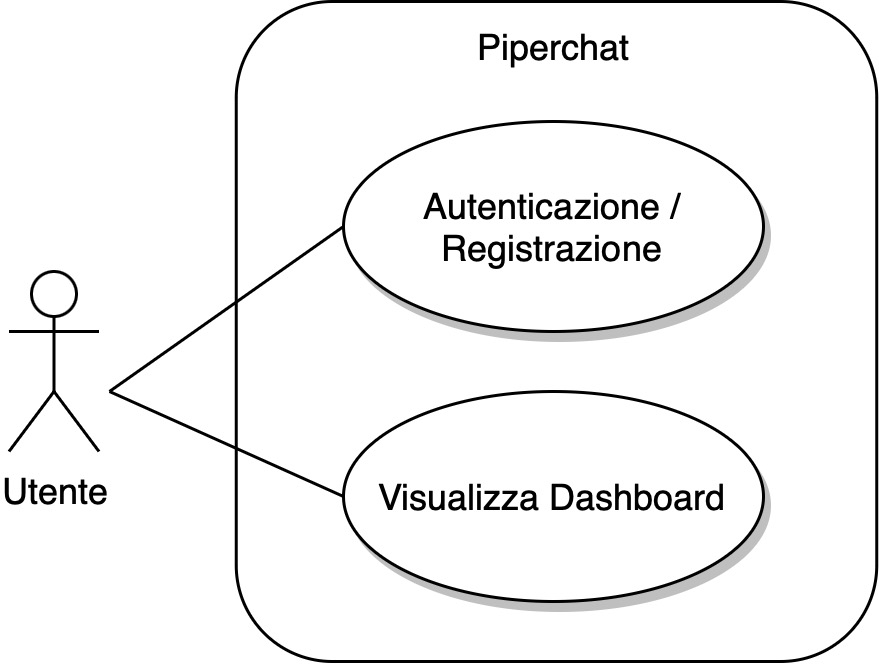
\includegraphics[width=0.6\linewidth]{sections/01-goal/img/use-cases/piperchat-Casi d'uso-1.jpg}
    \caption{Diagramma dei casi d'uso di un utente non autenticato}
\end{figure}

%
%
%
\subsubsection{Utente autenticato}

Dopo aver eseguito l'autenticazione, un utente acquisisce la possibilità di svolgere numerose azione, che riguardano diversi ambiti.
%
Si possono identificare i seguenti scenari:

\begin{enumerate}
    \item L'utente ha ora possibilità di gestire il proprio profilo ed è abilitato a ricevere le notifiche a lui indirizzate.

    \item L'utente può utilizzare la gestione delle richieste di amicizia che prevede di poter 
        \begin{enumerate*}
            \item inviarne ad altri utenti,
            \item accettare le richieste ricevute
            \item rifiutare le richieste ricevute.
        \end{enumerate*}
        
    \item L'utente ha la possibilità di creare server oppure partecipare a server già creati.
\end{enumerate}

\begin{figure}[H]
    \centering
    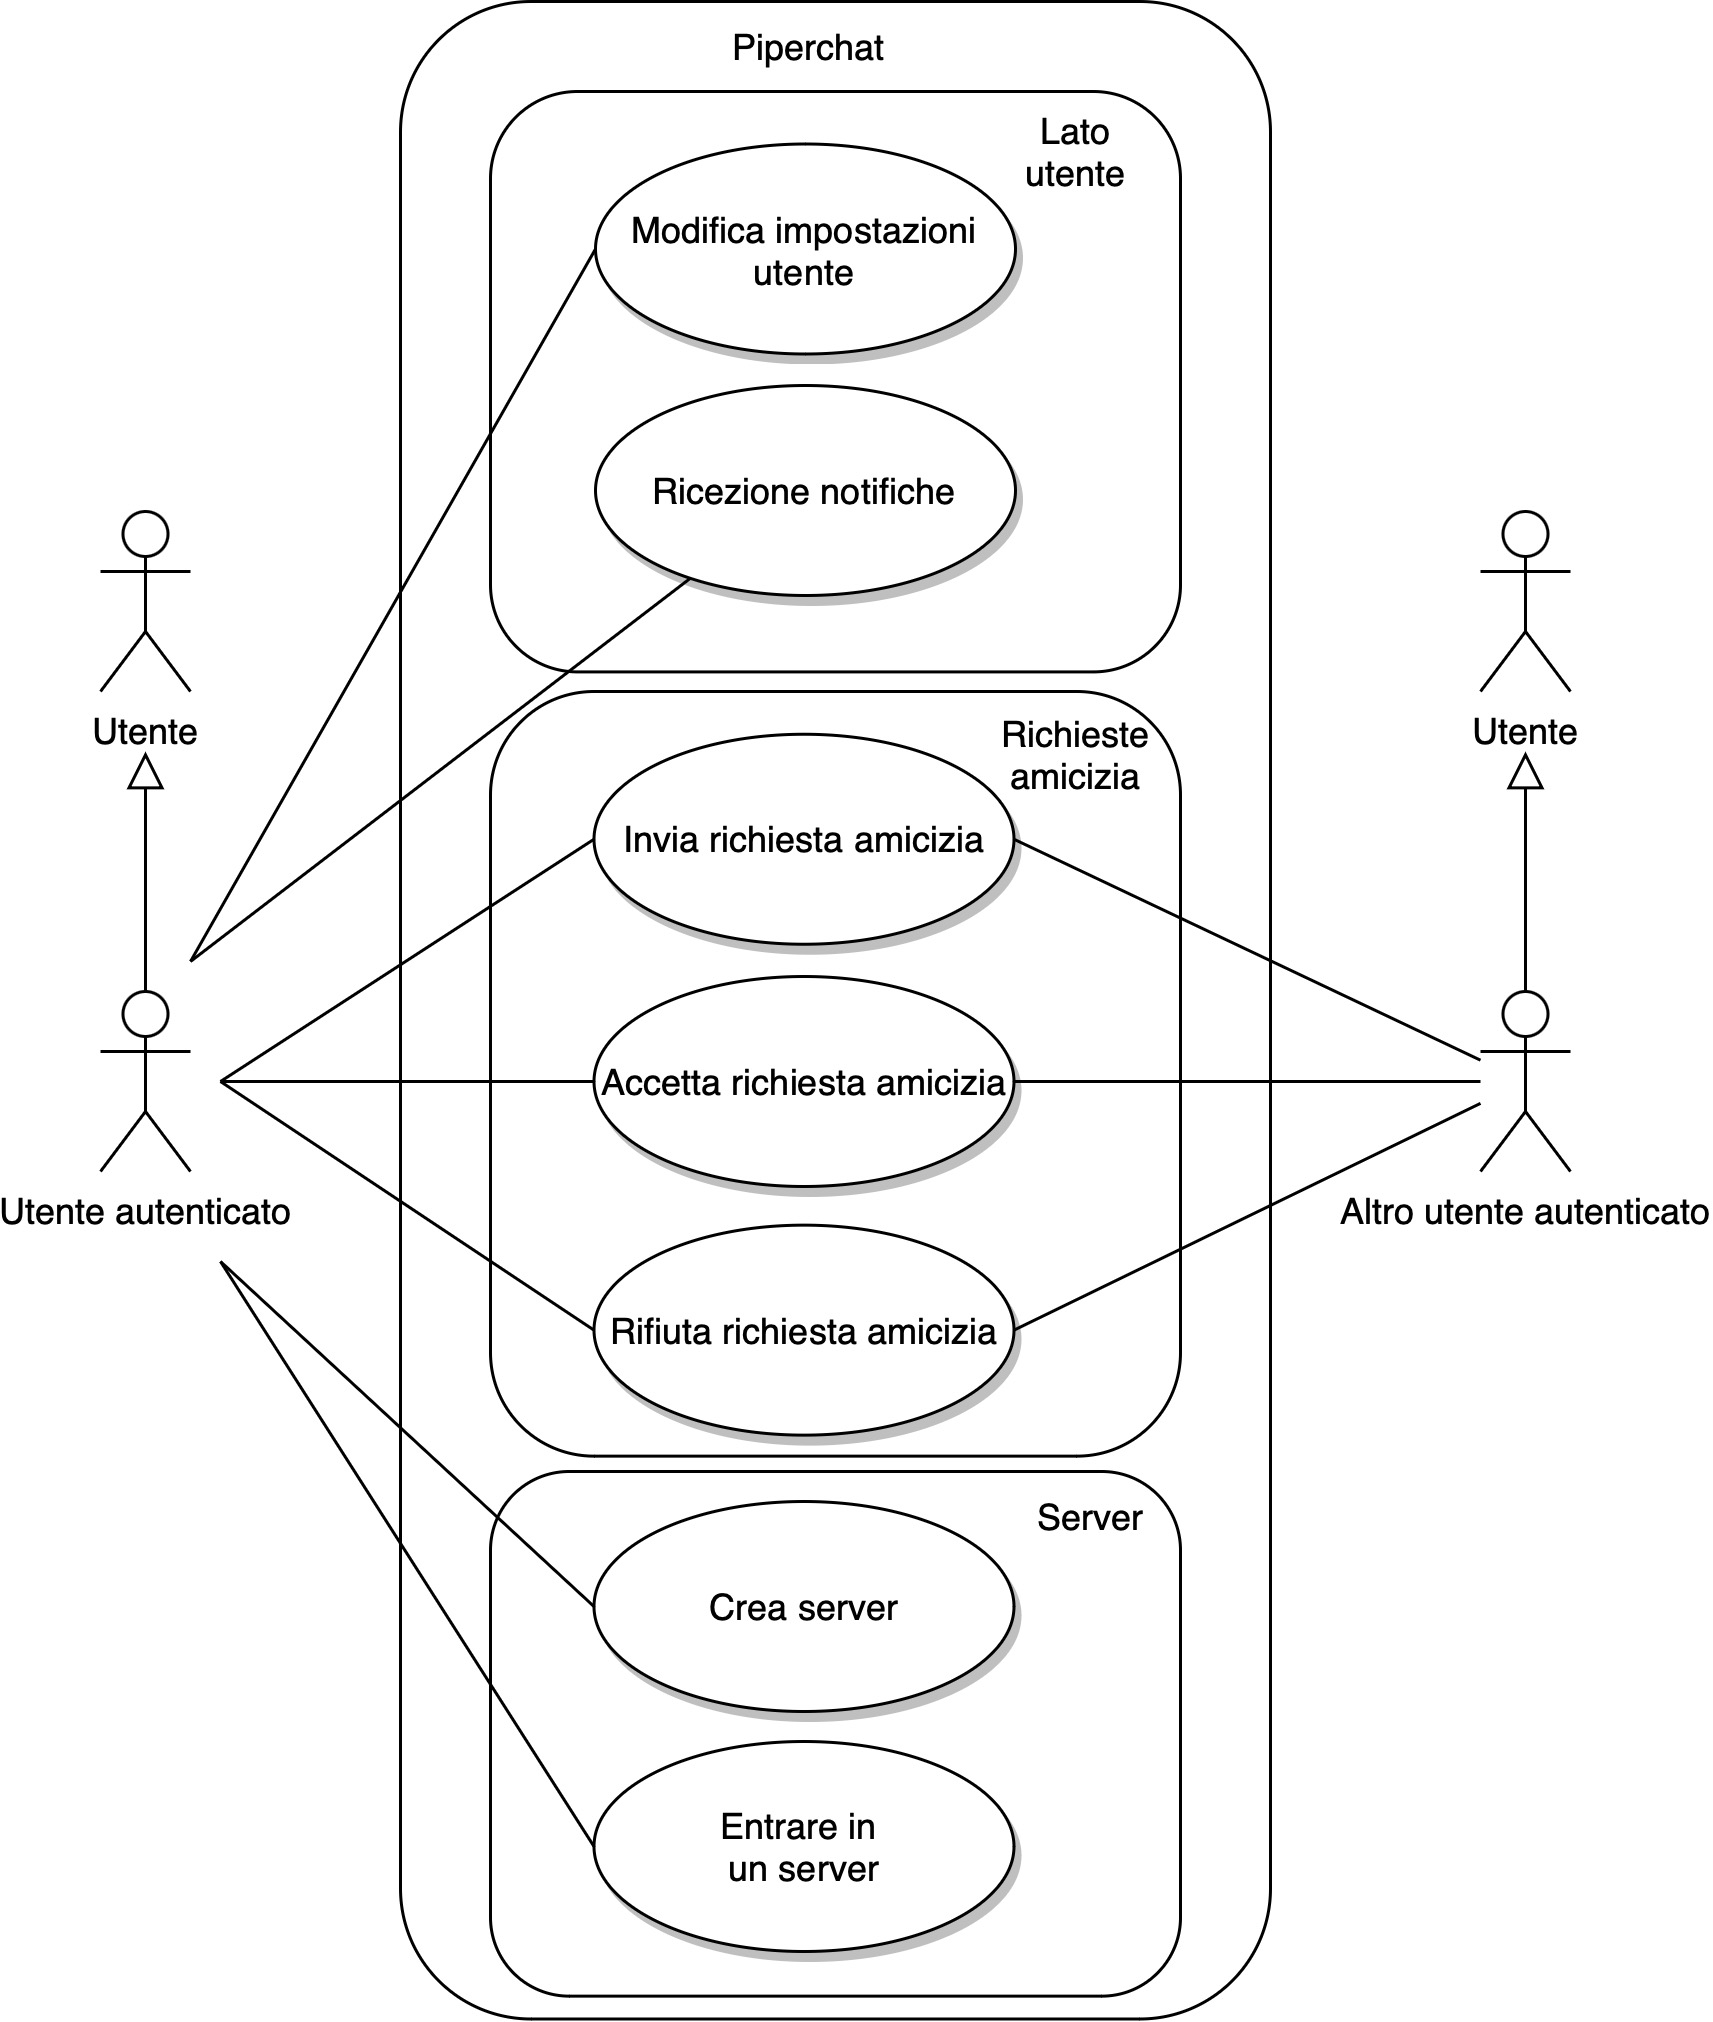
\includegraphics[width=1\linewidth]{sections/01-goal/img/use-cases/piperchat-Casi d'uso-2.jpg}
    \caption{Diagramma dei casi d'uso di un utente autenticato}
\end{figure}

%
%
%
\subsubsection{Utente amministratore di server}

Un utente, dopo aver creato un server, ne diventa amministratore.
%
Questo permette di accedere alle funzionalità di gestione per esso, tra le quali si possono evidenziare le seguenti:

\begin{enumerate}
    \item L'amministratore può aggiornare le informazioni del server o eliminarlo.

    \item L'amministratore può rimuovere un utente dal server.

    \item L'amministratore può creare i canali (testuali o multimediali).

    \item L'amministratore può aggiornare o rimuovere i canali già creati.
\end{enumerate}

\begin{figure}[H]
    \centering
    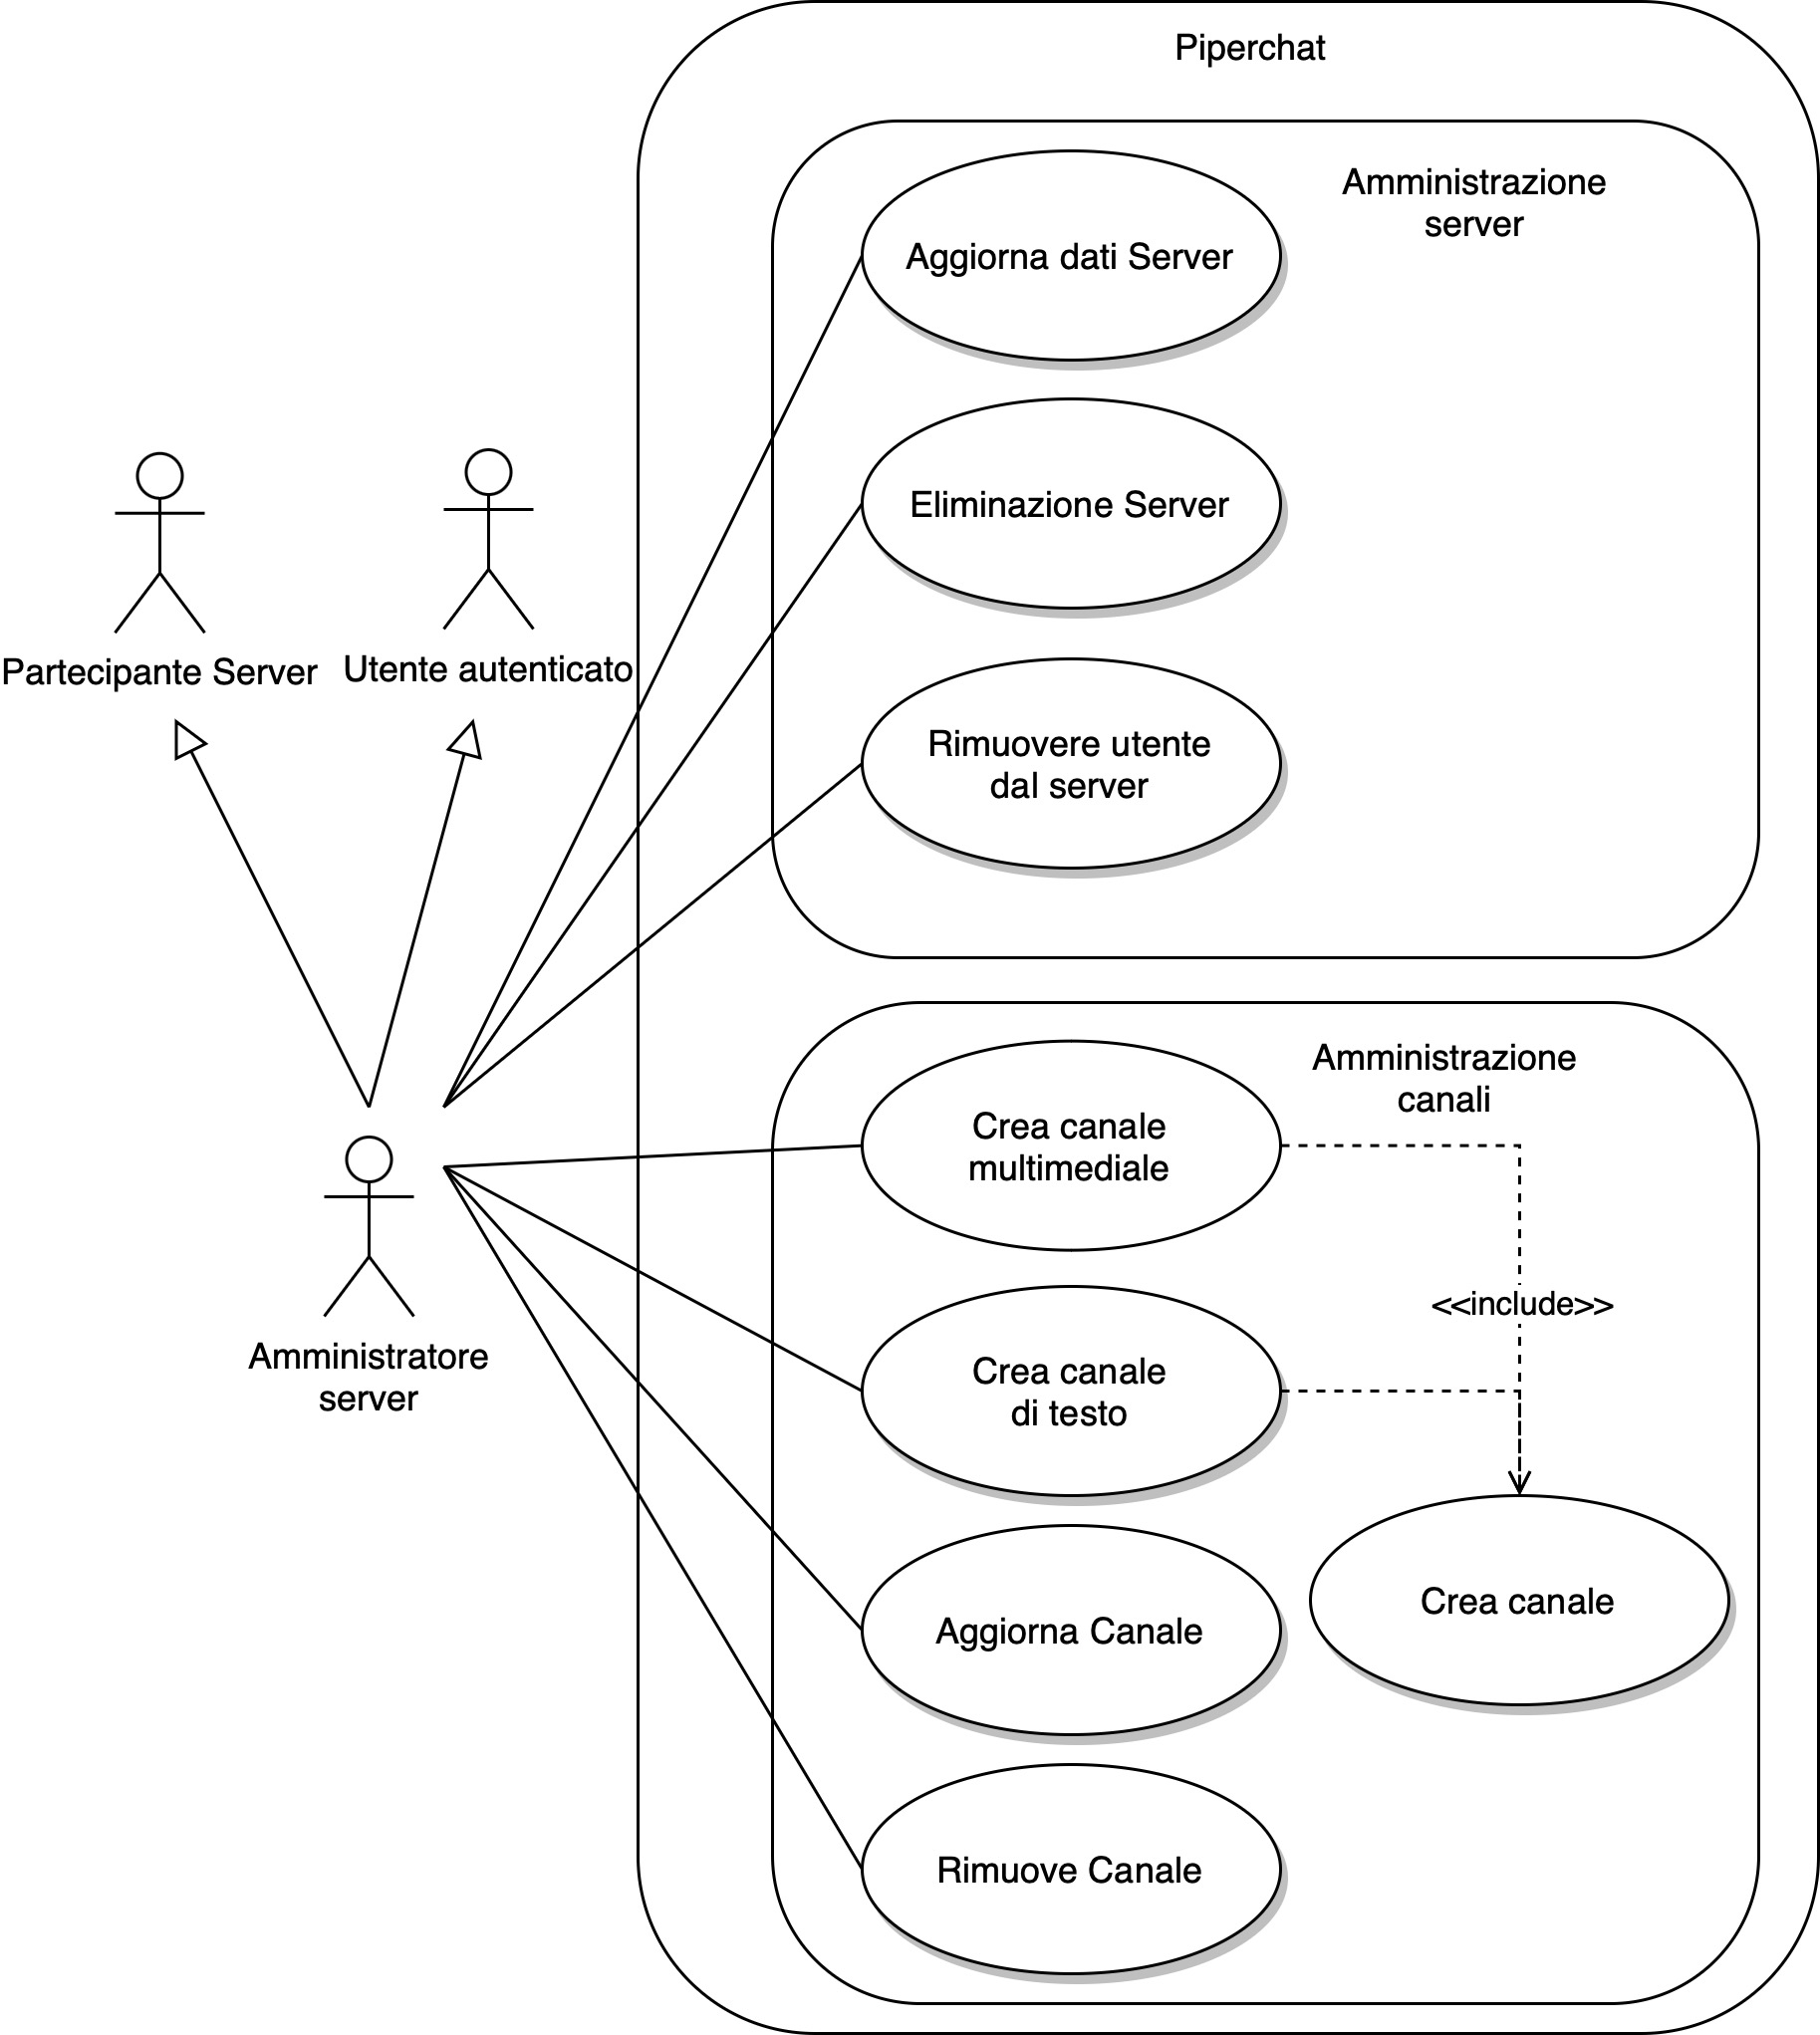
\includegraphics[width=1\linewidth]{sections/01-goal/img/use-cases/piperchat-Casi d'uso-3.jpg}
    \caption{Diagramma dei casi d'uso di un utente amministrazione di un server}
\end{figure}

%
%
%
\subsubsection{Interazione tra utente e amici}

Due utenti, dopo aver stretto amicizia, hanno la possibilità di interagire fra loro nei seguenti modi:

\begin{enumerate}
    \item Inviare messaggi all'interno della chat tra i due utenti.

    \item Partecipare alla sessione multimediale.
\end{enumerate}

\begin{figure}[H]
    \centering
    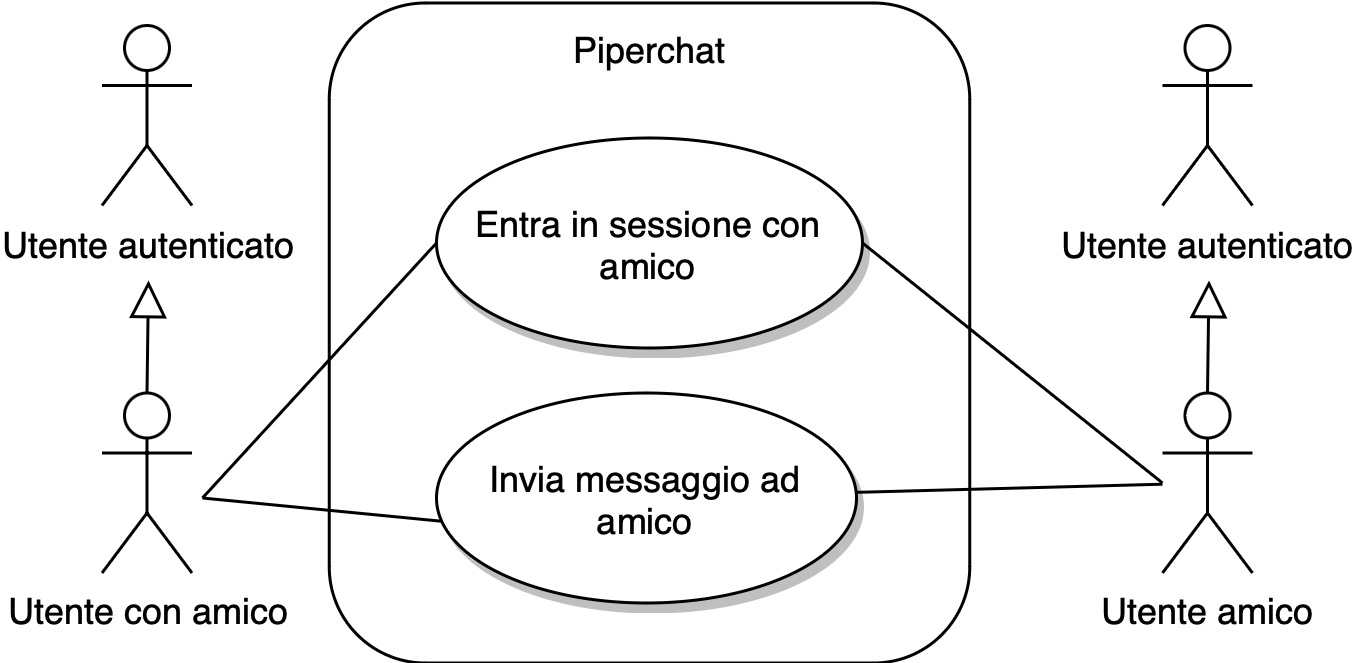
\includegraphics[width=1\linewidth]{sections/01-goal/img/use-cases/piperchat-Casi d'uso-4.jpg}
    \caption{Diagramma dei casi d'uso di un utente che interagisce con un amico}
\end{figure}

%
%
%
\subsubsection{Interazione di un utente partecipante ad un server}

Un utente che partecipa ad un server ha la possibilità di interazione attraverso i canali che sono stati creati, nei quali può:

\begin{enumerate}
    \item Inviare messaggi all'interno dei canali testuali.

    \item Partecipare ad un sessione in un canale multimediale.
\end{enumerate}

\begin{figure}[H]
    \centering
    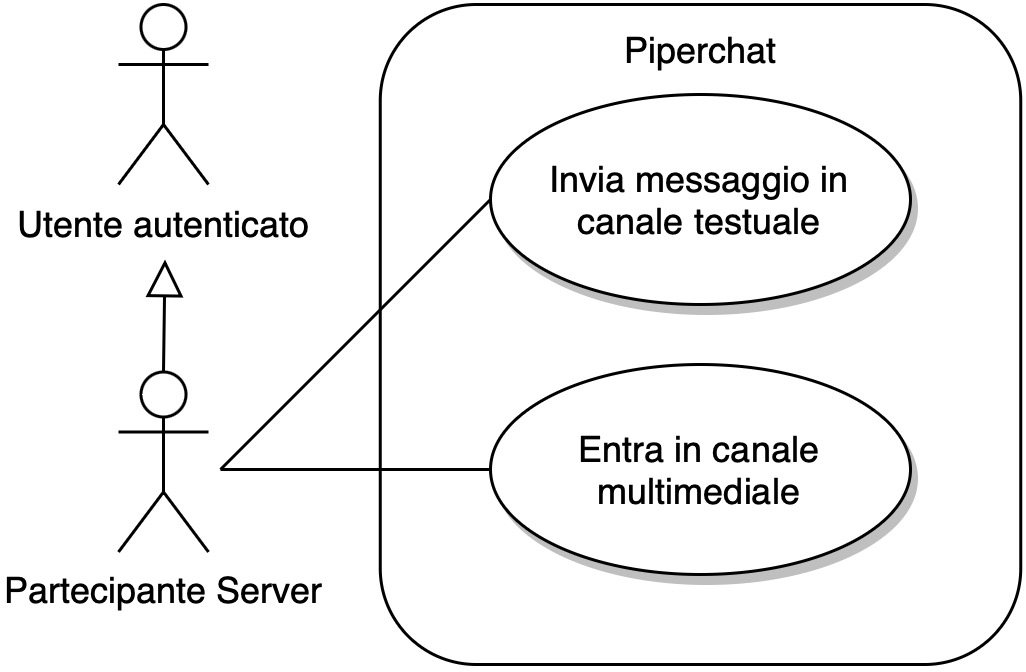
\includegraphics[width=0.6\linewidth]{sections/01-goal/img/use-cases/piperchat-Casi d'uso-5.jpg}
    \caption{Diagramma dei casi d'uso di un utente che partecipa ad un server}
\end{figure}

%
%
%
\subsubsection{Utente in sessione multimediale}

Un utente in sessione multimediale, sia in una privata con un amico, che in un canale, ha la possibilità di gestire microfono e webcam e di uscire dalla sessione stessa.

\begin{figure}[H]
    \centering
    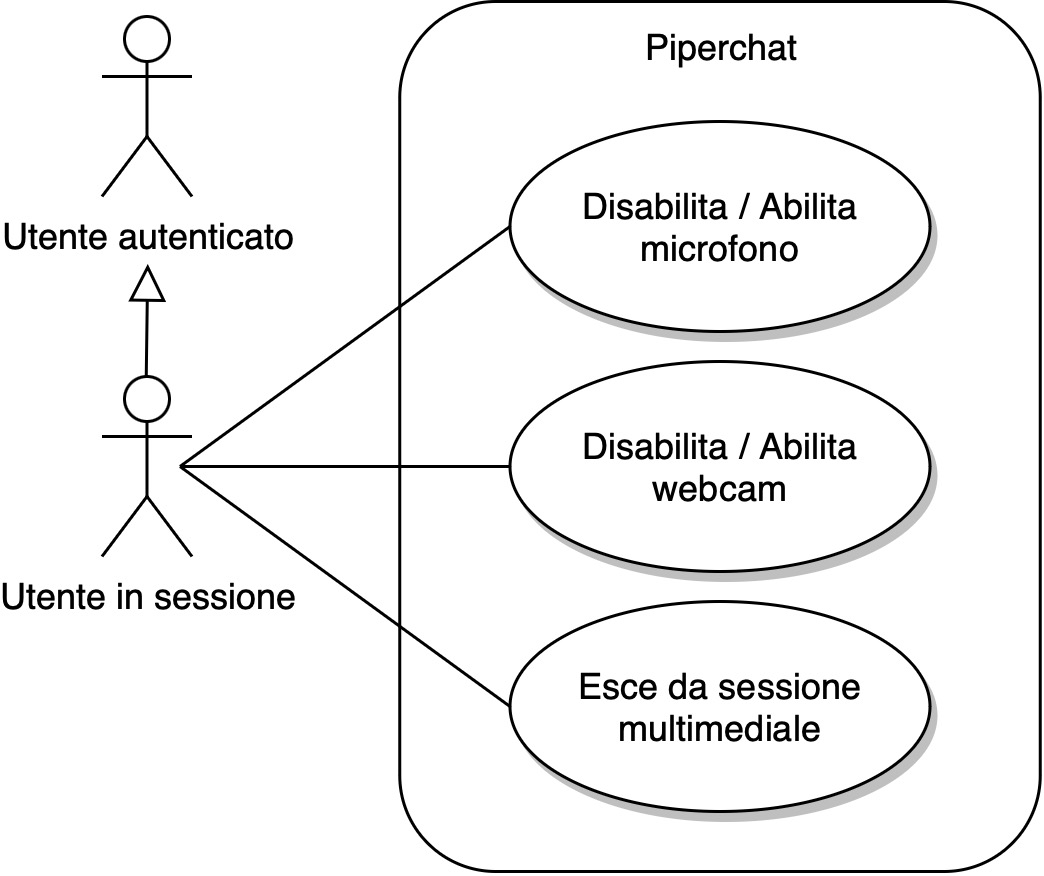
\includegraphics[width=0.7\linewidth]{sections/01-goal/img/use-cases/piperchat-Casi d'uso-6.jpg}
    \caption{Diagramma dei casi d'uso di un utente che partecipa ad una sessione}
\end{figure}

% \begin{figure}[H]
%     \centering
%     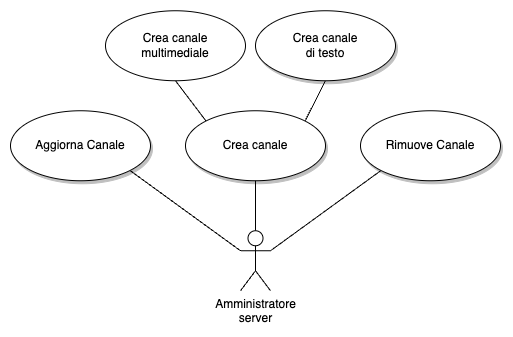
\includegraphics[width=0.7\linewidth]{sections/01-goal/img/use-cases/piperchat-Casi d'uso-9.drawio.png}
%     \caption{Caso d'uso di un utente amministratore di un server}
% \end{figure}

% \begin{figure}[H]
%     \centering
%     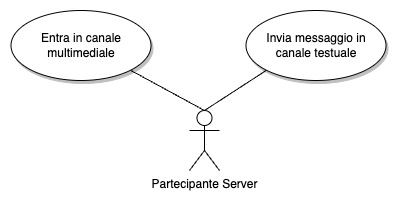
\includegraphics[width=0.7\linewidth]{sections/01-goal/img/use-cases/piperchat-Casi d'uso-10.drawio.png}
%     \caption{Caso d'uso di un utente partecipante di un server}
% \end{figure}

% \begin{figure}[H]
%     \centering
%     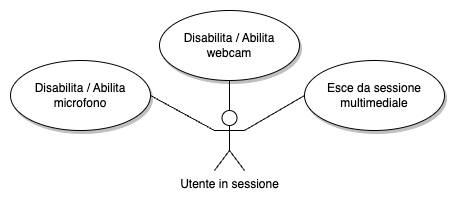
\includegraphics[width=0.7\linewidth]{sections/01-goal/img/use-cases/piperchat-Casi d'uso-6.drawio.png}
%     \caption{Caso d'uso di un utente in una sessione multimediale}
% \end{figure}

%
%
%
\subsection{Politica di autovalutazione}

%\begin{itemize}
%    \item How should the \emph{quality} of the %\emph{produced software} be assessed?
%    
%    \item How should the \emph{effectiveness} of the project %outcomes be assessed?
%\end{itemize}

Nella valutazione della \emph{qualità} del \emph{software prodotto} per il progetto \textit{PiperChat}, verrà adottato un approccio che tiene in considerazione i seguenti fattori:

\begin{itemize}
    \item \textbf{Funzionalità:} Le funzionalità principali del software, inclusi l'autenticazione degli utenti, la gestione delle amicizie, la messaggistica, la creazione di server e le funzionalità dei canali, devono essere implementate ed efficaci.

    \item \textbf{Affidabilità:} si valuterà la stabilità e l'affidabilità dell'architettura a microservizi, garantendo una comunicazione e un'interazione senza intoppi tra i diversi componenti.

    \item \textbf{Scalabilità:} 
    %la capacità del sistema di gestire una base utenti in crescita e un'attività crescente sarà un elemento chiave. 
    verrà valutato se l'applicazione avrà la capacità di gestire l'aumentare del carico computazionale legato all'aumentare degli utenti, le interazioni degli stessi, server e canali. Si terrà in considerazione la possibilità di scalabilità orizzontale indipendente del singolo microservizio in modo da consentire una gestione efficiente delle risorse.
    %e una risposta flessibile alle variazioni di carico mirate.

    \item \textbf{Sicurezza:} per quanto concerne gli aspetti di sicurezza, renderemo necessaria l'autenticazione nelle richieste, per garantire la riservatezza e l'integrità delle informazioni degli utenti.

\end{itemize}

Per valutare l'\emph{efficacia} degli esiti del progetto, verranno considerati i seguenti criteri:

\begin{itemize}

    \item \textbf{Decomposizione efficace:} verrà verificata la corretta decomposizione delle funzionalità in microservizi, garantendo che ciascun servizio abbia un ambito ben definito e che le interazioni tra i microservizi siano gestite in modo consono.

    \item \textbf{Dipendenze minime tra Microservizi:} si cercherà di minimizzare le dipendenze tra i microservizi, favorendo l'indipendenza e la modularità per semplificare la gestione e favorire la manutenibilità.

    \item \textbf{Reattività agli Eventi:} verrà assicurata una risposta pronta agli eventi attraverso l'implementazione di meccanismi di \emph{event-driven architecture} tra i microservizi e verso gli utenti finali.

    % \item \textbf{Scalabilità Indipendente:} si valuterà la capacità di ciascun microservizio di scalare indipendentemente dagli altri, consentendo una gestione efficiente delle risorse e una risposta flessibile alle variazioni di carico mirate.

    \item \textbf{Monitoraggio:} verrà implementato un sistema robusto di monitoraggio per i microservizi, permettendo di osservare l'attuale stato dei microservizi in gioco.
    
    %una rapida individuazione e risoluzione dei problemi, nonché una comprensione dettagliata delle attività del sistema.

\end{itemize}
